\documentclass[a4paper]{report}
\usepackage{amsfonts} % natural, complex, real, etc \mathbb
\usepackage{bussproofs}
\usepackage{listings}
\usepackage{fullpage}
\usepackage{stmaryrd} % llbracket rrbracket
\usepackage{MnSymbol} %\lcirclearrowleft
\usepackage{appendix}
\usepackage{color}
\usepackage[pdf]{pstricks} % pstrick environment
\usepackage{graphicx} % scalebox
\usepackage{glossaries}
\usepackage{rotating} % sidewaystable\c

\newcommand{\comm}[1]{[\textcolor{red}{#1}]}
\newcommand{\lang}[0]{\mathcal{L}}
\newcommand{\locus}[1]{\widetilde{#1}}
\newcommand{\pro}[0]{\textcolor{green}{+}~}
\newcommand{\cons}[0]{\textcolor{red}{-}~}
\newcommand{\even}[0]{\textcolor{blue}{=}~}
\newcommand{\gmarker}[1]{\textcolor{green}{~~~~~#1}}
\newcommand{\bmarker}[1]{\textcolor{blue}{~~~~~#1}}
\newcommand{\sq}{\vdash}
\newcommand{\bcell}[1]{\begin{minipage}{5cm}#1\end{minipage}}
\newcommand{\scell}[1]{\begin{minipage}{5cm}#1\end{minipage}}
\definecolor{dkred}{rgb}{0.5,0,0}
\definecolor{purple}{rgb}{0.58,0,0.82}
\definecolor{ltgrey}{rgb}{0.95,0.95,0.95}

\lstdefinelanguage{scheme}{
	backgroundcolor=\color{ltgrey},
	basicstyle=\color{black}\ttfamily\footnotesize,
	frame=single,
	showspaces=false,
	showstringspaces=false,
	showtabs=false,
	tabsize=4,
	stringstyle=\color{purple}\ttfamily\footnotesize,
	string=[b]{"},
	comment=[l];,
	commentstyle=\color{blue}\ttfamily\footnotesize
}

\lstdefinelanguage{java}{
	backgroundcolor=\color{ltgrey},
	basicstyle=\color{black}\ttfamily\footnotesize,
	frame=single,
	showspaces=false,
	showstringspaces=false,
	showtabs=false,
	tabsize=4,
	stringstyle=\color{purple}\ttfamily\footnotesize,
	string=[b]{"},
	comment=[l]//,
	commentstyle=\color{blue}\ttfamily\footnotesize
}

\lstdefinelanguage{code}{
	backgroundcolor=\color{ltgrey},
	basicstyle=\color{black}\ttfamily\footnotesize,
	frame=single,
	showspaces=false,
	showstringspaces=false,
	showtabs=false,
	tabsize=4,
	stringstyle=\color{purple}\ttfamily\footnotesize,
	string=[b]{"},
	comment=[l]//,
	commentstyle=\color{blue}\ttfamily\footnotesize
}

\lstdefinelanguage{shell}{
	backgroundcolor=\color{black},
	basicstyle=\color{white}\ttfamily\footnotesize,
	frame=single
	showspaces=false,
	tabsize=4,
	showstringspaces=false,
	showtabs=false
}

\lstnewenvironment{scheme}{\lstset{language=scheme}}{}
\lstnewenvironment{lscheme}{\lstset{language=scheme}}{}
\lstnewenvironment{shell}{\lstset{language=shell}}{}
\lstnewenvironment{code}{\lstset{language=code}}{}
\lstnewenvironment{java}{\lstset{language=java}}{}
\lstnewenvironment{cansi}{\lstset{language=java}}{}
\lstnewenvironment{csharp}{\lstset{language=java}}{}
\lstnewenvironment{matlab}{\lstset{language=code}}{}
\lstnewenvironment{xml}{\lstset{language=code}}{}
\lstnewenvironment{python}{\lstset{language=code}}{}

\newcommand{\ischeme}[1]{\colorbox{white}{\lstinline[language=scheme]&#1&}} %[
\newcommand{\ilscheme}[1]{\colorbox{white}{\lstinline[language=scheme]&#1&}} %[
\newcommand{\icode}[1]{\colorbox{white}{\lstinline[language=scheme]&#1&}} %[
\newcommand{\icansi}[1]{\colorbox{white}{\lstinline[language=java]&#1&}} %[
\newcommand{\ijava}[1]{\colorbox{white}{\lstinline[language=java]&#1&}} %[
\newcommand{\icsharp}[1]{\colorbox{white}{\lstinline[language=java]&#1&}} %[
\newcommand{\imatlab}[1]{\colorbox{white}{\lstinline[language=code]&#1&}} %[
\newcommand{\ixml}[1]{\colorbox{white}{\lstinline[language=code]&#1&}} %[
\newcommand{\ipython}[1]{\colorbox{white}{\lstinline[language=code]&#1&}} %[
\newcommand{\proj}[0]{\downarrow}
\newcommand{\inst}[0]{\lcirclearrowleft}
\newcommand{\reftab}[1]{[Table \ref{#1}]}
\newcommand{\reffig}[1]{[Figure \ref{#1}]}

\newcommand{\ax}[1]% axiome in prooftree
{\AxiomC{$#1$}}
\newcommand{\unc}[1]% unary conlusion in prooftree
{\UnaryInfC{$#1$}}
\newcommand{\bic}[1]% binary conlusion in prooftree
{\BinaryInfC{$#1$}}
\newcommand{\tric}[1]% trinary conclusion in prooftree
{\TrinaryInfC{$#1$}}
\newcommand{\quic}[1]% 4-conclusion in prooftree
{\QuaternaryInf{$#1$}}
\newcommand{\drule}% display the rule (not with the environnement prooftreee)
{\DisplayProof}
\newcommand{\rref}[1]% right label in prooftree
{\RightLabel{(\ref{#1})}}
\newcommand{\lref}[1]% left label in prooftree
{\LeftLabel{(\ref{#1})}}

\title{Iterative Typing}
\author{Christophe, Laurent}
\date{\today}
\begin{document}

\chapter{Future works}


\section{Miscellaneous}

\paragraph{Validation}

\paragraph{Error report} Although having a great practical interest, error messages was not the focus of this thesis. For now, iterative typing settles for the locus that cannot be unified as error message. This message although useful to develop iterative typing has little meaning for the casual iterative programmer:
\begin{scheme}
(define evil (lambda (x)
               (if x
                   1
                   "foo")))
(concat (evil #t) "bar")
\end{scheme}
\begin{shell}
Type error: unification failed on: {a5 => String, a4 => Boolean, a3 => a6, a5 => Number, a3 => (a4 -> Number), a10 => String, a9 => String, a8 => String, a7 => Boolean}.
\end{shell}
By spotting errors earlier than dynamically typed languages, iterative typing has a good potential to help the programmer to finds the right piece of code that must be fixed. Here is an algorithm that would exploit the specificities of iterative typing:
\begin{enumerate}
\item \emph{An other branch is viable}: we must blame the predicate and investigate why it has a wrong value.
\item \emph{No other other branch is viable}: we are in a dead end, the previous dynamic events have to be pointed out.
\end{enumerate}

\paragraph{Constraints simplification} For now, type constraints inserted in LScheme code contain all the details of the Hindley-Milner inference. As a result even simple procedure like \ischeme{map} a huge amount of type constraint. For instance the classic evil case:
\begin{scheme}
(define evil (lambda (x)
               (if x
                   1
                   "foo")))
(concat (evil #t) "bar")
\end{scheme}
Is currently compiled into:
\begin{lscheme}
(define evil (lambda (x)
               (if x
                   [{a8 => Number, a6 => (a7 -> Number), a13 => String, a12 => String, a11 => String, a10 => Boolean} 1]
                   [{a8 => String, a6 => (a7 -> String), a13 => String, a12 => String, a11 => String, a10 => Boolean} "foo"])))
(concat ([evil {a8 => String, a7 => Boolean, a6 => a9}] #t) "bar")
\end{lscheme}
When the below LScheme code would have suffice:
\begin{lscheme}
(define evil (lambda (x)
               (if x
                   [a => Number}  1]
                   [{a => String} "foo"])))
(concat ([evil {a => String}] #t) "bar")
\end{lscheme}

\paragraph{Continuation} The behavior of continuations inside an iterative framework has not been investigated so far. However, as the interpreter is free of side effect, we believe the support of continuations will not be problematic.

\paragraph{User-defined type} The \ischeme{struct} keyword basically adds a new type on the type system which does not require any core modifications. Constructor, accessors and mutators must be automatically generated.

\paragraph{Assignments} Although begin very permissive, iterative typing does not allow to modify the type of a variable. Fixed typed variable is the base of any static type system. However, we still have hoop to implement assignment with a different type. For instance, we could consider assignments as dynamic events and let the locus could encapsulate the type modification at runtime.


\chapter{H}

\section{Hindley-Milner Inference}

\paragraph{Introduction} The Hindley Milner type inference is crucial practically and thorically\comm{ref necessary}. It is the fundation of languages like ML and Haskell \comm{ref necessary}. The language itself is very close to $\lang$ \reftab{hml}.

\begin{table}
\centering
\begin{tabular}{|r|l|l|}
\hline
$e$ & $x$ & Identifier\\
& $(e\ e')$ & Application\\
& $(\lambda x . e)$ & Abstraction\\
& $(let\ x=e\ in\ e')$ & Polymorphic binding\\
\hline
\end{tabular}
\caption{Grammar that generates the language used in the Hindley Milner type inference.}
\label{hml}
\end{table}

\paragraph{Semantic value} 
\begin{itemize}
\item $B_0, \ldots,B_N$ is a list of set of values.
\item $W=\{w\}$ is the singleton of failure.
\item $V=B_0\cup\ldots\cup B_N\cup W\cup F$ where $F=V\times F$
\end{itemize}
The semantic function return a semantic value from an expression and an environment: $\epsilon\in HM\times (Id\to V)\to V$. This function is really close to the semantic function of the $\lang$ language \cite{hm1}.

\paragraph{Typed semantic value}
\begin{enumerate}
\item Monotype:
	\begin{itemize}
	\item $v:\beta_i\Leftrightarrow v\in B_i$
	\item $v:\mu_1\to\mu_2\Leftrightarrow \forall v':\mu_1.((v\ v'):\mu_2\vee (v\ v')=w$
	\end{itemize}
\item Polytype: $v:\tau$ means that for every monotype instance $\mu$ of $\tau$ we have: $v:\mu$.
\item Type scheme: $v:\sigma$ means that for every generic instance $\tau$ of $\sigma$ we have : $v:\tau$
\end{enumerate}
$A\vDash e:\sigma$ means that $\epsilon\ \llbracket e\rrbracket\ \eta:\sigma$ where $x:\sigma' \in A\Rightarrow \eta\ x:\sigma'$. 

\paragraph{Type and Interpretation} The type set is identical as the one used for iterative typing \reftab{hmt}. The semantic function $\epsilon$ is very close to the one of $\lang$ \cite{hm1}. 

\begin{table}
\centering
\begin{tabular}{|r|l|}
\hline
$\tau$ & $\beta$\\
\hline
$\tau$ & $\tau \to \tau$\\
\hline
$\sigma$ & $\forall x . \tau$\\
\hline
\end{tabular}
\caption{The grammar that generate the polymorphic type given a set of primitive type $\mu$ and an infinite set of type variables $x$ ~\cite{damas}.}
\label{hmt}
\end{table}

\paragraph{Type system} The Hindely Milner type inference is based on the type system \reffig{hmts}. That type system define the steps that must follow a derivation, $A\vdash e:\sigma$ means that there exists a derivation that leads to that 

\begin{figure}
\begin{tabular}{cc}
$$\ax{}
\LeftLabel{[TAUT]}
\RightLabel{$(x:\sigma\in A)$}
\unc{A\vdash x:\sigma}
\drule$$
&
$$\ax{A\vdash e:\sigma}
\LeftLabel{[SUB]}
\RightLabel{$(\sigma\geq\sigma')$}
\unc{A\vdash e:\sigma'}
\drule$$
\\
$$\ax{A\vdash e:\sigma}
\LeftLabel{[GEN]}
\RightLabel{$\alpha$ not free in $A$}
\unc{A\vdash e:\forall\alpha\sigma}
\drule$$
&
$$\ax{A\vdash e:\tau'\to\tau}
\ax{A\vdash e'\to \tau'}
\LeftLabel{[COMB]}
\bic{A\vdash (e\ e'):\tau}
\drule$$
\\
$$\ax{A_x\cup\{x:\tau'\}\vdash e:\tau}
\LeftLabel{[ABS]}
\unc{A\vdash (\lambda x.e):\tau'\to\tau}
\drule$$
&
$$\ax{A\vdash e:\sigma}
\ax{A_x\cup\{x:\sigma\}\vdash e':\tau}
\LeftLabel{[LET]}
\bic{A\vdash(let\ x=e\ in\ e'):\tau}
\drule$$
\end{tabular}
\caption{The Hindely Milner type system \cite{hm2}. $A_x$ represent a set of assumptions without any assumption on $x$.}
\label{hmts}
\end{figure}

\begin{figure}
\centering
$$
\ax{}
\LeftLabel{[TAUT]}
\unc{(x:\alpha)\vdash(x:\alpha)}
\LeftLabel{[ABS]}
\unc{\vdash (\lambda x.x):\alpha\to\alpha}
\LeftLabel{[GEN]}
\unc{\vdash (\lambda x.x):\forall \alpha (\alpha\to\alpha)}
\drule$$
\caption{A derivation of the identity function.}
\label{derivid}
\end{figure}

\paragraph{Soundness} $A\vdash e:\sigma\Rightarrow A\vDash e:\sigma$

\paragraph{Algorithm} The Hindley-Milner inference algorithm is prooven to be soundness and complete (respectively to its associated type system):
\begin{enumerate}
\item Soundness: $W(A,e)$ succeed with $(S,tau)$ then there exists a derivation $SA\vdash e:\tau$.
\item Completeness (with $A'$ instance of $A$): if there exists a derivation such that: $A'\vdash e: \sigma$ then
	\begin{enumerate}
	\item $W(A,e)$ succeed
	\end{enumerate}
\end{enumerate}

\paragraph{Example} Here is a small example that use the identity function under its polymorphic form:
\begin{scheme}
(let id (lambda (x) x)
  (cat-num (id "yo") (id 1)))
\end{scheme}
\begin{enumerate}
\item The first expression which is inferenced is \ischeme{(lambda (x) x)} which is obviously of type: $a\to a$ (simple monomorphic evalution).
\item The body of the let expression can now be analyzed knowing that $cat-num :: [String~Numeral \to Numeral]$ and that  $id :: \forall a . a \to a$ (first rule).
	\begin{itemize}
	\item $([String~Numeral \to String] ([b \to b]~String) ([c \to c]~Numeral))$ (second rule).
	\item $([String~Numeral \to String] String~Numeral)$ (monomorphic inference).
	\item $String$ (monomorphic inference).
	\end{itemize}
\end{enumerate}


\chapter{MISC}
\subsection{Why don't we want polymorphic let?}
$(let evil (lambda (x) (if x 1 "yo")) (+ (evil \#t) (evil \#f)))$ $evil (lambda (x :: bool) (if x 1 "yo") :: b) :: Bool \to b$ We loose dynamicity otherwise dico plumbery.
\subsection{Execution \& free variables}
Linked variable describe a type: $(lambda (x) x) :: \forall a. a \to a$ ; when free variables represent an incertainty: $(if (eq? x 0) 1 "yo") :: a$ or $(lambda (x) x :: a) :: \forall a . a \to a$ : in the body of the lambda, $a$ represent an incertainti, we don't know what is the type of the argument. So during execution we carry around a generic instantiation which link all the free variable to concrete type (concrete type = type without free variable).
\subsection{Pure lambda calculus}
We have to complicate the language in order to accept some important construction of the lambda calculus (cf fix \& let).

\chapter{Actual work}

\section{Standard monomorphic type system}

\begin{equation}
\ax{x : \tau \in \Gamma}
\unc{\Gamma \vdash x : \tau}
\drule 
\end{equation}

\begin{equation}
\ax{\Gamma \vdash e_1 : \tau}
\ax{\Gamma \vdash e_2 : \tau\to\tau'}
\bic{\Gamma\vdash (e_1 e_2) : \tau'}
\end{equation}

\begin{equation}
\ax{\Gamma, x:\tau\vdash e:\tau'}
\unc{\Gamma \vdash (\lambda x. e) : \tau \to \tau'}
\end{equation}

\begin{equation}
\ax{\Gamma\vdash e:\tau}
\ax{\tau' \leq \tau}
\bic{\Gamma\vdash e:\tau}
\end{equation}



\chapter{Introduction}
\chapter{Context}
Quest to find errors as soon as possible.

\chapter{Technic}

\section{Introduction}

\section{Input}
\subsection{Semantic}
\begin{itemize}
\item $B_i$ is a CPO of primitive semantic value. The minium element of $B_i$ is named $\bot_i$. For instance $B_{byte}=\{0,1,2,3,4,5,6,7\}$ ;  $\bot_{byte}=0$.
\item $B_0=T=\{true,false,\bot_T\}$ where $\bot_T \leq true$ and $\bot_T \leq false$.
\item $W=\{wrong\}$ is the singleton of the failure semantic.
\item $V = B_0 + ... + B_N + F + W$ where $F = V \to V$ is the set of the functions from $V$ to $V$. The minimum element of $V$ is named $\bot_V$.
\end{itemize}
\subsection{Language}
\begin{tabular}{|l|r|}
\hline
$E$ & $x$\\
& $[E E]$\\
& $[\lambda x.E]$\\
& $[if E E E]$\\
& $[let x E E]$\\
\hline
\end{tabular}
\subsection{Interpretation}

\section{Output}
\subsection{Semantic}
Let $\tilde W = W + \{\tilde{wrong}\}$ the extended failure semantic. Further we will see that $wrong$ represents a static failure when $\tilde{wrong}$ represents a dynamic failure. The semantic of the output language is given by: $\tilde V = B_0 + ... + B_N + F + \tilde W$ (so $\tilde V = V + \{\tilde{wrong}\}$). 
\subsection{Language}
\begin{tabular}{|l|r|}
\hline
$E$ & $\{x \tau\}$\\
& $\{[E E] \tau\}$\\
& $\{[\lambda x.E]\tau\}$\\
& $\{[if E \rho E\rho E]\tau\}$\\
\hline
\end{tabular}
\subsection{Interpretation}


\chapter{YOOO}

\begin{tabular}{|l|r| }
\hline
$E$ & $x \tau$\\
& $[E E] \tau$\\
& $[\lambda x.E]\tau$\\
& $[if E p E p E]$\\
\hline
\end{tabular}

\begin{itemize}
\item $inter(x\tau,env)=env(x)$
\item $inter([e_1 e_2]\tau,env)=cond $
\end{itemize}

\chapter{Iterative typing}

\section{Semantic}

\section{Type}

\section{Language}
\subsection{Type system (well typed word)}


\section{An algorithm to find well typed word}

\chapter{Related workds}

\section{Interative typing}


\section{Hindley Milner rule system}

\begin{equation}
\ax{x:\sigma\in\Gamma}
\ax{\sigma\leq\tau}
\bic{\Gamma\sq x:\tau}
\drule
\end{equation}

\begin{equation}
\ax{\Gamma\sq e_0:\tau\to\tau'}
\ax{\Gamma\sq e_1:\tau}
\bic{\Gamma\sq e_0 e_1 : \tau'}
\drule
\end{equation}

\begin{equation}
\ax{\Gamma,x:\tau\sq e:\tau'}
\unc{\Gamma\sq\lambda x.e:\tau\to\tau'}
\drule
\end{equation}

\begin{equation}
\ax{\Gamma\vdash e_0:\tau}
\ax{\Gamma,x:\Gamma'(\tau)\vdash e_1:\tau'}
\bic{\Gamma\vdash let x = e_0 in e_1:\tau'}
\drule
\end{equation}

\section{Soft Typing}
\begin{tabular}{|r|l|}
\hline
P & num\\
& nil\\
& cons T T\\
& ->\\
& N\\
\hline
Ps & P Ps\\
& $\epsilon$\\
\hline
N & (not num)\\
& (not nil)\\
& (not cons)\\
& (not ->)\\
\hline
T & + Ps\\
T & + Ps X\\
\hline
Ts & T Ts\\
& $\epsilon$\\
\hline
\end{tabular}

\begin{itemize}
\item Soft typing
\item Gradual typing ~\cite{a}
\end{itemize}

\chapter{Idea, implication}

\section{Extended language}

$G : Env \to Bool$

\begin{tabular}{|r|l|}
\hline
$E$ & $x$\\
& $[E E]$\\
& $[E E \tau]$\\
& $[if\ E\ g E\ g \tau]$\\
& $[\lambda x.E]$\\
& $[let\ x=E\ in\ E]$\\
\hline
$C$ & $[E]$\\
\hline
\end{tabular}

\chapter{Evaluation}
\chapter{Conclusion}

\chapter{Annexe}

\section{Complte partial order}

Here is the definition of partial order set (poset):

$$poset (A,\leq) := \left\{\begin{array}{l}
	\forall a\in A . a \leq a\\
	\forall a_1, a_2 \in A . (a_1 \leq a_2 \cup a_2\leq a_1) \Rightarrow a_1 = a_2\\
	\forall a_1, a_2, a_3 \in A . (a_1 \leq a_1 \cup a_2\leq a_3) \Rightarrow a_1 \leq a_2\\
	\end{array}\right.$$

A complete partial order is a poset in which each directed subset has a supremum.

$$cpo (A,\leq) := \left\{\begin{array}{l}
	poset (A,\leq)\\
	\forall \alpha \subseteq A. (\alpha \neq \varphi \cup \forall x,y \in \alpha \exists z\in \alpha . (x,y \leq z)) \Rightarrow \exists z\in A . (\forall x \in \alpha z \leq x)\end{array}\right.$$

\section{Hindley Milner}

\subsection{Semantic}

\paragraph{Semantic values} A program deals with values, here we are about to define the set of all those value.

\begin{itemize}
\item $B_i$ is a CPO of primitive semantic value. The minium element of $B_i$ is named $\bot_i$. For instance $B_{byte}=\{0,1,2,3,4,5,6,7\}$ ;  $\bot_{byte}=0$.
\item $B_0=T=\{true,false,\bot_T\}$ where $\bot_T \leq true$ and $\bot_T \leq false$.
\item $W=\{wrong\}$ is the singleton of the failure semantic.
\item $V = B_0 + ... + B_N + F + W$ where $F = V \to V$ is the set of the functions from $V$ to $V$. The minimum element of $V$ is named $\bot_V$.
\end{itemize}

Then we define three relations:
\begin{enumerate}
\item $\rhd \in V \times \{B_0, ..., B_N, F, W\} \to T$:
	\begin{itemize}
	\item $v \in D \Rightarrow v \rhd D = true$
	\item $(v \notin D) \cup (v = \bot_V) \Rightarrow v \rhd D = \bot_T$
	\item $(v \notin D) \cup (v \neq \bot_V) \Rightarrow v \rhd D = false$
	\end{itemize}
\item $| \in V \times \{B_0, ..., B_N, F, W\} \to V$
	\begin{itemize}
	\item $v \in D \Rightarrow v | D = v$
	\item $v \notin D \Rightarrow v | D = \bot_d$
	\end{itemize}
\item $cond \in T \times V \times V \to V$
	\begin{itemize}
	\item $cond(true,v,v') = v$
	\item $cond(fase,v,v') = v'$
	\item $cond(\bot_T,v,v') = \bot_V$
	\end{itemize}
\end{enumerate}

\subsection{Syntaxic}

Lets $Id$ be the set of the identifiers ; $x$ ranges over $Id$. Lets $Exp$ be the language generated by the grammar:

\begin{tabular}{|r|l|}
\hline
$E$ & $x$\\
& $[E\ E]$\\
& $[if\ E\ E\ E]$\\
& $[\lambda x.E]$\\
& $[let\ x\ =\ E\ in\ E]$\\
\hline
\end{tabular}

\subsection{Link}

\paragraph{Environement} The environement function allow to link identifier to semantic value: $Env = Id \to V$. We can modify an environement with the function: $\{/\} \in Env \times Id \times V \to Env$ such that:
\begin{itemize}
\item $env\{v/x\}(x)=v$
\item $x \neq\tilde x \Rightarrow env\{v/\tilde x\}(x) = env(x)$
\end{itemize}

\paragraph{Semantic function} $inter : Exp \to Env \to V$: the semantic function is actually an interpreter.

\begin{itemize}
\item The interpretation of an identifier is its mapping over the environement.
$$inter(x,env)=env(x)$$
\item The interpretation of an application is the result of the function discribed by the first expression given the argument described by the second expression. The interpretation is poluted by checks to ensure the first expression represent indeed a function from $V$ to $V$ and to ensure the evaluation of the argument has not failed. 
$$\begin{array}{rl}
inter ([e_1\ e_2],env) = cond & inter(e_1,env)\rhd F\\
& \begin{array}{rl}
	cond & inter(e_2,env) \rhd W\\
	     & wrong\\
	     & (inter(e_1,env) | F)(inter (e_2,env))\\
	\end{array}\\
& wrong\\
\end{array}$$
\item
$$\begin{array}{rl}
inter([if\ e_1\ e_2\ e_3],env) = cond & inter(e_1,env) \rhd T\\
& \begin{array}{rl}
 	cond & inter(e_1,env)|T\\
 	     & inter(e_2,env)\\
 	     & inter(e_3,env)\\
	\end{array}\\
& wrong\\
\end{array}$$
\item $$inter([\lambda x.e],env)=\lambda v.inter(e,env\{v/x\})$$
\item $$\begin{array}{rl}
inter([let\ x=e_1\ in\ e_2],env)=cond & inter(e_1,env)\rhd W\\
& wrong\\
& inter(e_2,env\{inter(e_1,env)/x\})\\
\end{array}$$
\end{itemize}

\subsection{Type}

\paragraph{Monotype} For each $B_i$ we have a primitive type $\iota_i$. $\iota$ is used to range over $\{\iota_0,...,\iota_N\}$. Here is the grammar that generate the monotype language:
\begin{tabular}{|r|l|}
\hline
$\mu$ & $\iota$\\
& $\mu \to \mu$\\
\hline
\end{tabular}

\begin{itemize}
\item $v : \iota_i \Leftrightarrow (v=\bot_V \cap v \in B_i)$
\item $v:\mu_1 \to\mu_2\Leftrightarrow (v=\bot_V \cap ((\tilde v : \mu_1)\Rightarrow(v|F)(\tilde v):\mu_2 ))$
\end{itemize}

Some values has no monotype ($wrong$) and some others have mutliple monotypes ($\bot_T$, $[\lambda x. x]$).

We can proove that:
\begin{itemize}
\item $\forall v_1,v_2 \in V.(v_1:\mu \cap v_1 \leq v_2) \Rightarrow v_2 :\mu$
\item $(X \mbox{directed subset of} V)\Rightarrow (\forall x \in X. ??? dafuq$
\end{itemize}

\paragraph{Type} Now we introduce a set of variable. $\alpha$, $\beta$ and $\gamma$ are used to range over the type variables (we call type that contain variables polytype). Here is the grammar that generate the type language (which is ranged by $\tau$):
\begin{tabular}{|r|l|}
\hline
$\tau$ & $\iota$\\
& $\alpha$\\
& $\tau \to \tau$\\
\hline
\end{tabular}

$\tau_1\leq\tau_2$ means that we can obtain $\rho_1$ by replacing some of the variables of $\tau_2$ with types. We can now lift the type belongship to polytype: $v:\tau \Leftrightarrow \forall \mu \leq \tau. v:\mu$. Directly we have:

\begin{itemize}
\item $(v:\tau\cap \tilde\tau\leq \tau)\Rightarrow v:\tilde \tau$
\item $(v:\tau_1\to\tau_2 \cap)$
\end{itemize}



%%%%%%%%%%%%%%%%%%%%%%%%%%%%%%%%%%%%%%%%%%%%
%%%%%%%%%%%%%%%%%%%%%%%%%%%%%%%%%%%%%%%%%%%%
%%%%%%%%%%%%%%%%%%%%%%%%%%%%%%%%%%%%%%%%%%%%
%%%%%%%%%%%%%%%%%%%%%%%%%%%%%%%%%%%%%%%%%%%%
%%%%%%%%%%%%%%%%%%%%%%%%%%%%%%%%%%%%%%%%%%%%
%%%%%%%%%%%%%%%%%%%%%%%%%%%%%%%%%%%%%%%%%%%%
%%%%%%%%%%%%%%%%%%%%%%%%%%%%%%%%%%%%%%%%%%%%
%%%%%%%%%%%%%%%%%%%%%%%%%%%%%%%%%%%%%%%%%%%%
%%%%%%%%%%%%%%%%%%%%%%%%%%%%%%%%%%%%%%%%%%%%
%%%%%%%%%%%%%%%%%%%%%%%%%%%%%%%%%%%%%%%%%%%%
%%%%%%%%%%%%%%%%%%%%%%%%%%%%%%%%%%%%%%%%%%%%
%%%%%%%%%%%%%%%%%%%%%%%%%%%%%%%%%%%%%%%%%%%%
%%%%%%%%%%%%%%%%%%%%%%%%%%%%%%%%%%%%%%%%%%%%
%%%%%%%%%%%%%%%%%%%%%%%%%%%%%%%%%%%%%%%%%%%%
%%%%%%%%%%%%%%%%%%%%%%%%%%%%%%%%%%%%%%%%%%%%
%%%%%%%%%%%%%%%%%%%%%%%%%%%%%%%%%%%%%%%%%%%%
%%%%%%%%%%%%%%%%%%%%%%%%%%%%%%%%%%%%%%%%%%%%
%%%%%%%%%%%%%%%%%%%%%%%%%%%%%%%%%%%%%%%%%%%%

% Some dynamic languages

\begin{itemize}
\item \emph{JavaScript}: multi-paradigm and weakly typed language which has first call procedure and that is used as the Internet assembly language. Which make it the world most used language. Although \emph{JavaScript} took a lot of name and convention from \emph{Java} those two languages are somehow unrelated, \emph{JavaScript} is far more inspired from \emph{Scheme}. 
\item \emph{Python}: multi-paradigm language most successfully used to create prototypes.
\item \emph{Perl}: high-level, general purpose language ; initially developed as a scripting language for Unix.
\item \emph{Smalltalk}: pure reflexive object-oriented language developed in the seventies, heavily used nowadays thanks to web application frameworks like \emph{Seaside}.
\item \emph{Ruby}: multi-paradigm reflexive language combine \emph{Smalltalk} feature with a syntax inspired of \emph{Perl}. Also heavily used again through a web application framework: \emph{Ruby on Rail}.
\item \emph{Scheme}: dialect of Lisp developed in the seventies by the MIT that considers procedure as first citizen and support current continuation. This language is known to provide great power within a minimalist design which make it suitable for learning purpose and experimentations.
\end{itemize}

%%%%%%%%%%%%%%%%%%%%%%%%%%%%%%%%%%%%%%%%%%%%
%%%%%%%%%%%%%%%%%%%%%%%%%%%%%%%%%%%%%%%%%%%%
%%%%%%%%%%%%%%%%%%%%%%%%%%%%%%%%%%%%%%%%%%%%
%%%%%%%%%%%%%%%%%%%%%%%%%%%%%%%%%%%%%%%%%%%%
%%%%%%%%%%%%%%%%%%%%%%%%%%%%%%%%%%%%%%%%%%%%
%%%%%%%%%%%%%%%%%%%%%%%%%%%%%%%%%%%%%%%%%%%%
%%%%%%%%%%%%%%%%%%%%%%%%%%%%%%%%%%%%%%%%%%%%
%%%%%%%%%%%%%%%%%%%%%%%%%%%%%%%%%%%%%%%%%%%%
%%%%%%%%%%%%%%%%%%%%%%%%%%%%%%%%%%%%%%%%%%%%
%%%%%%%%%%%%%%%%%%%%%%%%%%%%%%%%%%%%%%%%%%%%
%%%%%%%%%%%%%%%%%%%%%%%%%%%%%%%%%%%%%%%%%%%%
%%%%%%%%%%%%%%%%%%%%%%%%%%%%%%%%%%%%%%%%%%%%
%%%%%%%%%%%%%%%%%%%%%%%%%%%%%%%%%%%%%%%%%%%%
%%%%%%%%%%%%%%%%%%%%%%%%%%%%%%%%%%%%%%%%%%%%
%%%%%%%%%%%%%%%%%%%%%%%%%%%%%%%%%%%%%%%%%%%%
%%%%%%%%%%%%%%%%%%%%%%%%%%%%%%%%%%%%%%%%%%%%
%%%%%%%%%%%%%%%%%%%%%%%%%%%%%%%%%%%%%%%%%%%%
%%%%%%%%%%%%%%%%%%%%%%%%%%%%%%%%%%%%%%%%%%%%

In the guarding process, typing use a set whom each element (named type) is associate to a subset of the semantic domain. In term of typing we would say that \icode{+} expects two numbers and returns a number ; the execution \icode{1 + "foo"} would then produce a type error because \icode{"foo"} is a string (is associate to the type string). The type set construction is dependent of the used typing technique.

\paragraph{Typing} Typing is about providing guards for a large class of bad configuration. Informally typing is the discipline that ensure a program's execution has a meaning and does not apply operations on irrelevant data structures. 

In this chapter we will introduce the typing discipline, two of its main stream and a comparison between those. Then we will expose the working language of this thesis.

\section{Element of typing}

\paragraph{Introduction}  Firstly, through model simulation, we define the concepts of well-behaved execution and program safety. Then we introduce the type concept and two way to perform typing: dynamically and statically. Please notice that this presentation is very personal and informal.

\paragraph{Language, Semantic \& error} A language is specified by its grammar and its interpretation relatively to a semantic. The semantics regroup the values manipulates by the language, the interpretation function returns a semantic value from an expression and an environment. One important semantic values the "error" value which is used each time an unwanted configuration shows up. Here is a piece of code that perfectly respects the Java grammar but produces differents kind of errors:

Notice that the concept of error is interpretation dependent, for instance \icode{1 + "foo";} does not produce an error in Javascript specification. When a program does not never produce an error we say it is safe.

\paragraph{Typing} Is a strategy the provide guards for a large class of errors. Type errors are formally defined by the provided guards but generally type safety ensure that no operation are performed out of its definition domain. We can say that a typing ensure that an execution has a meaning. In the guarding process, typing use a set whom each element (named type) is associate to a subset of the semantic domain. In term of typing we would say that \icode{+} expects two numbers and returns a number ; the execution \icode{1 + "foo"} would then produce a type error because \icode{"foo"} is a string (is associate to the type string). The type set construction is dependent of the used typing technique.

\paragraph{Dynamic typing} One very direct way to provide type safety is to add type flag on any computed value. Then type checks are performed before applying any primitive operation:
\begin{code}
x = "foo"; // x points to bytes with the string type flag
x = 1;     // x points to bytes with the number type flag
x + 1;     // as both the values of x and 1 have the number
           // type flag, we are sure x + 1 is type safe
\end{code}
In dynamic typing, values are typed and variable can point to values of any type.

\paragraph{Static typing} Static typing is about easing the interpreter to ensure well-behavior. So before being executed, programs pass through a static type checker that either accept or reject the programs, the purpose of this pass is to provide assumptions for the interpretation. For instance the following Java programs is accepted by the static type checker, but it uses casting which involve the interpreter:
\begin{java}
Object[] array = new Object[3]; // array that can contain anything
array[0] = new Car();
array[1] = new Patato();
array[2] = new Car();
Car car = (Car) array[1];       // runtime error
car.drive();                    // undefined behavior
\end{java}
Static type checker attach type to variables and more generally to most expressions ; each variable has a fixed type and it is not possible to change it. The static type checkers are based on a set of syntactic rules named type system.



\paragraph{Type}  

Obvious error in symbolic programming may be hard to detect  symbolic programming  After compilation to machine code, obvious error may be hard to detect. For instance both  for instance both "1" Typing use the concept of type which represent the a subset of 


 ; for instance $1+"foo"$ and $1/0$ will result in an error in most interpreters. Errors can be detected in two places: the application of a primitive and the evaluation of a grammatical rule

The operators inside that semantic are generally not defined for the value of the domain ; for instance 



Hardwares only manipulate bit words through very low level operator like bit-adder. If we want to use this model to simulate the behavior of higher level model we first need to translate its value in term of bit words.



\paragraph{Model simulation} We define a model $(V,O)$, as a set of values and a set of operators that manipulate those values. Lets defined two models:
\begin{enumerate}
\item The algebra model: $\mathcal{A}=(\mathbb{N}^{100}\cup\{\top,\bot\},\{+,\vee\})$. This model manipulates boolean and ranged natural numbers trough the operators $+ : \mathbb{N}^{100}\times\mathbb{N}^{100}\to\mathbb{N}^{100}$ and $\vee :\{\top,\bot\}\times\{\top,\bot\}\to\{\top,\bot\}$. 
\item The binary model: $\mathcal{B}=(\{0,1\}^N,\{+,jump,push,...\})$. The binary model manipulates bit words through some low level operators. We present this model as the interface provided by some hardware.
\end{enumerate}
If we want our hardware working on the $\mathcal{A}$ model, we need to simulate the behavior of $\mathcal{A}$ with $\mathcal{B}$. The first step is to represent each value of $\mathcal{A}$ by values of $\mathcal{B}$. Then the $\mathcal{A}$ operators can be defined as combinations of $\mathcal{B}$ operators. But how can we translate the definition domain of the $\mathcal{A}$ operators? If we do not answer this question, the computation $1 + \bot$ may either crash, return an undefined result or produce an unsuspected side effect. Typing is about providing guard to prevent such computation ; an execution that does not produce such computation is said well behaved. A program that does only produce any well-behaved execution is said to be safe (effectively with IO actions, a program may produce a lot of different execution). Does two concept are very language dependent ; for instance $1 + "3"$ may be well-behaved in some languages (because an errors is thrown or an implicit cast is performed) and may be ill-behaved in some others. 

\paragraph{Type} Types attach meaning to binary representations, each specific domain of the simulated model is granted by a type which is used to ensure that the higher level operations are performed on rightful values. In the precedent model, both $1$ and $\bot$ has binary representations but the one of $1$ has the type $Number$ and the one of $\bot$ has the type $Boolean$. In order to ensure well-behaved execution, typing technique deduce types. The construction of the type set is very dependent of the used typing technique.

\paragraph{Dynamic typing} One very direct way to provide safety is to add type flag on any computed value. Then type checks are performed before applying any primitive operation:
\begin{code}
x = "foo"; // x points to bytes with the string type flag
x = 1;     // x points to bytes with the number type flag
x + 1;     // as both the values of x and 1 have the number
           // type flag, we are sure x + 1 is well-behaved
\end{code}
In dynamic typing, values are typed and variable can point to values of any type. The interpreter is the only responsible to ensure well-behavior. Insofar as dynamic typing reject all ill-behaved executions, all the programs are safe.

\paragraph{Static typing} Static typing is about easing the interpreter to ensure well-behavior. So before being executed, programs pass through a static type checker that either accept or reject the programs, the purpose of this pass is to provide assumptions for the interpretation. For instance the following Java programs is accepted by the static type checker, but it uses casting which involve the interpreter:
\begin{java}
Object[] array = new Object[3]; // array that can contain anything
array[0] = new Car();
array[1] = new Patato();
array[2] = new Car();
Car car = (Car) array[1];       // runtime error
car.drive();                    // undefined behavior
\end{java}
Static type checker attach type to variables and more generally to most expressions ; each variable has a fixed type and it is not possible to change it. The static type checkers are based on a set of syntactic rules named type system.



%%%%%%%%%%%%%%%%%%%%
%%%%%%%%%%%%%%%%%%%%
%%%%%%%%%%%%%%%%%%%%
% IDEA & IMPLICATION 3.1 dynamic language.


\paragraph{Introduction} As we known, a program without any extern interaction is deterministic and it is well-typed or ill-typed. But that class of program does hardly anything useful (as they return the same result at each execution), it is the IO actions that add practical interest to programs. IO actions may change the values that are manipulated from on execution to an other. That freedom combined with conditional structures allows to vary the applied set of instruction. So IO actions and conditional structure are complementary and give all the dynamic flavor to languages \reftab{comp_if_read}.

\begin{table}
\centering
\begin{tabular}{|p{3.5cm}|p{3.5cm}|p{3.5cm}|p{3.5cm}|}
\hline
&Conditional structures & IO actions & IO actions and\\
& & & conditional structure\\
\hline
Description & Execution is deterministic, nothing can change from one execution to an other. & Executions carry around different values and possibly types but the same instructions are executed each time. & Executions carry around different values and possibly types, different sets of instructions may be executed.\\
\hline
Restriction & Programs are reduced to calculators, there is not input just a result. & Recursion is impossible (no stopping condition). & \\
\hline
\end{tabular}
\caption{Complementary of IO actions and conditional structures.}
\label{comp_if_read}
\end{table}

\paragraph{Input as a trace}

\paragraph{Bad starting}

\paragraph{Wet dream}

\paragraph{A first compromise}

\paragraph{Wet dream} As we do not introduce time, we can model the inputs as a trace. We can model dynamic program as boxes that for a given trace may:
\begin{enumerate}
\item Terminate without error
\item Terminate with a type error.
\item Terminate with a value error.
\end{enumerate}
Given a program, computing the set of all the "good" trace that make it terminate without errors. So at the moment, the user goes out of the "good" traces the execution is stopped. If the set of the "good" trace is empty, the program is simply rejected. This would be the best scenario in term of expressiveness, safety and early detection.

\paragraph{A first compromise} Even if the set of value is practically finite, it is not realist to analyze each trace of values. So we must regroups the values. If those groups are defined by predicate we go to the dependent typing discipline which is out of the range of this thesis. If we split values into set we fall into a normal type semantic. As we are working with type we do no have access to value anymore. So conditional structure becomes dynamic event and we must analyze both branches (on specific case, type may suffice but we work on the general case, this can be an improvement) and we cannot detect value error anymore. For this series of dynamic event there is no type errors (but possibly value errors).

\begin{figure}
\centering
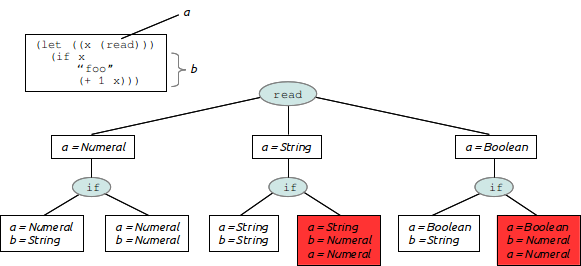
\includegraphics{images/type_state.png}
\caption{The different paths that may take the execution of a dynamic program.}
\label{type_state}
\end{figure}


\begin{scheme}
(let ((x (read))
      (y (read)))
  (if (equal? x y)
      (+ x x)               ; then branch
      (string-append y y))) ; else branch
\end{scheme}
Here are the following viable event sequence:
\begin{itemize}
\item $(String,String,else)$
\item $(Number,Number,then)$
\item $(Number,String,then)$
\item $(Number,String,else)$
\end{itemize}
With refined static analysis we would know that if the \ischeme{read} returned different type, the $then$ event cannot happen.

\paragraph{The iterative compromise} The first compromise let us an exponential growth on both read and if which is not acceptable \reffig{type_state}. In price of a little bit more computation at runtime, the iterative typing propose almost the same feature. The idea is this: knowing the precedent dynamic event we can know of the current event is about to lead the trace out of the viable one.

\begin{scheme}
(let ((x (read))
      (y (read)))
  (if (equal? x y)
      (+ x x)               ; then branch
      (string-append y y))) ; else branch
\end{scheme}
Here are the following viable event sequence:
\begin{itemize}
\item First \ischeme{read}: no constraint
\item Second \ischeme{read}: no constraint
\item \ischeme{if}: if predicate is satisfied, the first \ischeme{read} must have returned a $Number$. If the predicate is not satisfied then the second \ischeme{read} must have returned a $String$.
\end{itemize}
We detect errors a little bit latter, with the first compromise if both \ischeme{read} would returned a $Boolean$ we would directly detect the error (without waiting the next event).


%%%%%%%%%%%%%%%%%%%%%%%%
% 3.2 Iterative typing %
%%%%%%%%%%%%%%%%%%%%%%%%

\paragraph{Compilation} So iterative typing is capable to tell at each dynamic event if the program will produce a type error until the next event. To achieve this, a variant of the Hindley-Milner type inference is used.
\begin{itemize}
\item The type of a dynamic event (either \ischeme{if} or \ischeme{read}) is a type variable.
\item The type variable introduced on \ischeme{read} call are stored on the identifier.
\item The constraints done inside a conditional branch are stored in the head of the branch.
\end{itemize}
\begin{itemize}
\item Lets take back our last example:
\begin{scheme}
(let ((x (read))
      (y (read)))
  (if (equal? x y)
      (+ x x)
      (string-append y y)))
\end{scheme}
\item Following our inferencer it would be compiled in something like this:
\begin{scheme}
(let ((x (read [a]))
      (y (read [b])))
  (if (equal? x y)
      [a=Numeral]
        (+ x x)
      [b=String ]
        (string-append y y)))
\end{scheme}
\end{itemize}

\paragraph{Interpretation} We must keep a trace of the precedent events to decide the viability of the current event. Those informations are stored inside a set of type constraint that we carry trough the execution. Such a set is called locus.
\begin{itemize}
\item For the inputs \ischeme{1} and \ischeme{"foo"} the compiled program returns \ischeme{"foofoo"}. Here is the evolution of the locus through the execution:
\begin{scheme}
(let ((x (read [a]))          ; [a=Numeral]
      (y (read [b])))         ; [a=Numeral, b=String]
  (if (equal? x y)
      [a = Numeral]            
        (+ x x)
      [b = String ]           ; [a=Numeral, b=String, b=String]
        (string-append y y))) ; [a=Numeral, b=String]
\end{scheme}
\item For the inputs \ischeme{1} and \ischeme{2} the compiled program returns a type error. Here is the evolution of the locus through the execution:
\begin{scheme}
(let ((x (read [a]))          ; [a=Numeral]
      (y (read [b])))         ; [a=Numeral, b=Numeral]
  (if (equal? x y)
      [a = Numeral]            
        (+ x x)
      [b = String ]           ; [a=Numeral, b=Numeral, b=String]
        (string-append y y))) ; TYPE ERROR
\end{scheme}
\end{itemize}

\paragraph{An other point of view} As the inference goes on, it introduce type variable and as much freedom degrees. When an application is analyzed, type constraint are generated that restrict the number of type the type variables may takes. We store those constraint trough the program ans we just must ensure at least one instantiation is possible. The word locus comes from the fact that it define a "place" where type variable may be instantiated. 


\begin{table}
\centering
\begin{tabular}{|c|c|l|l|}
\hline
Constructor & Arity & $\lang$ expression & An associated monotypes \\
\hline
$String$ & 0 & $"foo"$ & $String$\\
\hline
$Boolean$ & 0 & $true$ & $Boolean$\\
\hline
$Number$ & 0 & $3.14$ & $Number$\\
\hline
$\to$ & 2 & $(\lambda\ (x)\ x)$ & $\xi\to\xi$ \\
& & $(\lambda\ (x)\ (if\ (<\ x\ 0)\ "pos"\ "neg"))$ & $Number\to String$\\
\hline
$[]$ & 1 & $(cons\ 1\ (cons\ 2\ (cons\ 3\ null)))$ & $[Number]$\\
& & $null$ & $[String]$\\
\hline
$(.)$ & 2 & $(pair\ 1\ "foo")$ & $(Number.String)$\\
\hline
\end{tabular}
\caption{The different type constructor currently implemented in the iterative prototype. Notice that the action of associate types to expressions has not been defined, the examples are just meant to develop an intuitive interpretation of monotypes.}
\label{pract_type_constr}
\end{table}

%%%%%%%%%%%%%%%%%%%%%%%
% A stupid derivation %
%%%%%%%%%%%%%%%%%%%%%%%

\chapter{Garbage}

We should demonstrate that any program can be derivated, can only crash at locus intersections or unsafe primitives like car divide,... 

\section{The $\locus\lang$ type system}

\paragraph{Judgment} The judgments of the $\locus\lang$ type system are little bit more elaborated than the ones of $\lang$. Judgments have to form: $A|L\vdash e:\sigma$, intuitively it means: from the assumptions $A$ and relatively to the locus $L$ we can deduce that the expression $e$ has the type $\sigma$. This dichotomy of the hypotheses ($A$ is transformed to $A|L$) allows us to introduce scopes for generated type constraints. And that is exactly what we need to express the conditional structures in an iterative way.

\begin{table}
\centering
$$\boxed{\begin{array}{c}\begin{array}{cc}
\\
\ax{A_x\cup\{x:\tau\}\vdash e:\tau'}
\LeftLabel{ABS}
\unc{A\vdash(\lambda x.e):\tau\to\tau'}
\drule
&
\ax{A\vdash e:\tau'\to\tau}
\ax{A\vdash e':\tau'}
\LeftLabel{APP}
\bic{A\vdash (e\ e'):\tau}
\drule
\\\\\\
\ax{\{x:\sigma\}\in A}
\LeftLabel{ID}
\unc{A\vdash x:\sigma}
\drule
&
\ax{A\vdash x:\sigma}
\ax{\textcolor{red}{\tau}\sqsubseteq\sigma}
\LeftLabel{\textcolor{red}{SUB}}
\bic{A\vdash (\textcolor{red}{\sigma}\ \textcolor{red}{\tau}\ x):\textcolor{red}{\tau}}
\drule
\\\\\\
\ax{A\vdash e:\sigma}
\ax{A_x\cup\{x:\sigma\}\vdash e':\tau'}
\LeftLabel{LET}
\bic{A\vdash (let\ e\ e'):\tau'}
\drule
&
\ax{A_x\cup\{\tau\to\tau'\}\vdash e:\tau\to\tau'}
\LeftLabel{REC}
\unc{A\vdash (rec\ x\ e):\tau\to\tau'}
\drule
\\\\\\
\ax{c::\gamma}
\LeftLabel{CONST}
\unc{A\vdash c:\gamma}
\drule
&
\ax{A\vdash e:\tau}
\ax{A\vdash x:\tau}
\LeftLabel{ASSIGN}
\bic{A\vdash (set\ x\ e):\tau}
\drule
\end{array}
\\\\\\
\ax{A\vdash e:\forall\xi_{1..i}.\tau\to\tau'}
\ax{\xi\notin free(A)}
\LeftLabel{GEN}
\bic{A\vdash e:\forall\xi,\xi_{1..i}.\tau\to\tau'}
\drule
\\\\\\
\ax{A\vdash e:\tau}
\ax{\{\xi_i'\mapsto\tau_i'\}A\vdash e':\tau'''}
\ax{\{\xi_i''\mapsto\tau_i''\}A\vdash e'':\tau'''}
\LeftLabel{\textcolor{red}{COND}}
\tric{A\vdash (if\ e\ \textcolor{red}{\{\xi_i'\mapsto\tau_i'\}}\ e'\ \textcolor{red}{\{\xi_i''\mapsto\tau_i''\}}\ e''):\tau'''}
\drule
\\\\
\end{array}
}$$
\caption{The $\locus\lang$ type system.}
\end{table}


\begin{table}
\centering
$$\begin{array}{c}
\ax{f:Number\to\xi_{if}\in\{f:Number\to\xi_{if},x:\xi\}}
\LeftLabel{ID}
\unc{\{f:Number\to\xi_{if},x:\xi\}\vdash f:Number\to\xi_{if}}
\ax{1::Number}
\LeftLabel{CONST}
\unc{\{f:Number\to\xi_{if},x:\xi\}\vdash 1:Number}
\LeftLabel{APP}
\bic{\{f:Number\to\xi_{if},x:\xi\}\vdash (f\ 1):\xi_{if}\ \ \ \ (1)}
\drule
\\\\\\
\ax{f:String\to\xi_{if}\in\{f:String\to\xi_{if},x:\xi\}}
\LeftLabel{ID}
\unc{\{f:String\to\xi_{if},x:\xi\}\vdash f:String\to\xi_{if}}
\ax{"foo"::String}
\LeftLabel{CONST}
\unc{\{f:String\to\xi_{if},x:\xi\}\vdash "foo":String}
\LeftLabel{APP}
\bic{\{f:String\to\xi_{if},x:\xi\}\vdash (f\ "foo"):\xi_{if}\ \ \ \ (2)}
\drule
\\\\\\
\ax{x:\xi\in\{f:\xi',x:\xi\}}
\LeftLabel{CONST}
\unc{\{f:\xi',x:\xi\}\vdash x:\xi}
\ax{(1)}
\ax{(2)}
\LeftLabel{COND}
\tric{\{f:\xi',x:\xi\}\vdash(if\ x\ \{\xi'\mapsto Number\to\xi_{if}\}\ (f\ 1)\ \{\xi'\mapsto String\to\xi_{if}\}\ (f\ "foo")):\xi_{if}}
\LeftLabel{ABS}
\unc{\{f:\xi'\}\vdash(\lambda x.(if\ x\ \{\xi'\mapsto Number\to\xi_{if}\}\ (f\ 1)\ \{\xi'\mapsto String\to\xi_{if}\}\ (f\ "foo"))):\xi\to\xi_{if}}
\LeftLabel{ABS}
\unc{\{\}\vdash(\lambda f.(\lambda x.(if\ x\ \{\xi'\mapsto Number\to\xi_{if}\}\ (f\ 1)\ \{\xi'\mapsto String\to\xi_{if}\}\ (f\ "foo")))):\xi'\to(\xi\to\xi_{if})}
\drule
\\
\end{array}$$
\caption{The $\locus\lang$ program: $(\lambda f.(\lambda x.(if\ x\ \{\xi'\mapsto Number\to\xi_{if}\}\ (f\ 1)\ \{\xi'\mapsto String\to\xi_{if}\}\ (f\ "foo"))))$ is type safe.}
\label{deriv_cond}
\end{table}

\paragraph{Overview} The entire $\locus\lang$ type system is presented at \reftab{locus_lang_type_system}. In the rest of this section we will justify each rule of this type system.

\paragraph{MONO-ID} This rule is fundamental, it allow to freely distribute a type between assumptions and locus. The big diffence between assumptions and loci is that informations stored on the assumptions rely on the program to be relaxed

Here is two derivation that end with: $x:String$
$$\begin{array}{c|c}
\ax{x:String\in\{x:String\}}
\LeftLabel{MONO-ID}
\unc{\{x:String\}|\{\}\vdash x:String}
\drule
&
\ax{x:\xi\in\{x:\xi\}}
\LeftLabel{MONO-ID}
\unc{\{x:\xi\}|\{\xi.String\}\vdash x:String}
\drule
\end{array}$$
Although those derivation end up with the same conclusion, the left one is much strict than the right one. That is because the assumptions

\paragraph{CONST and ASSIGN} Those rules are fairly simple are represent a direct adaption of the $\lang$ rules.

\paragraph{ABS and APP} The abstraction and application rule are very similar to the ones of $\lang$, they just carry a locus around. That is an important point, loci are not affected by abstraction neither applications. In comparison, it is those rules that carry most of the essence of gradual typing and soft typing. 

\paragraph{COND} The rule about the conditional structure motivate the dichotomy of the usual set of assumption. In essence: all the constraints stored inside the locus of a branch does not affect the rest of the inference. When all the information stored inside the assumptions must be shared by all the parts. In \reffig{if_deriv} we present a derivation that illustrate the behavior of the COND rule.

\begin{sidewaysfigure}
\centering
\begin{tabular}{c}
$$
\ax{f:\xi\to\xi\{f:\xi\to\xi,x:\xi'\}}
\LeftLabel{MONO-ID}
\unc{\{f:\xi\to\xi,x:\xi'\}|\{\xi.Number\}\vdash f:Number\to Number}
\ax{1::Number}
\LeftLabel{CONST}
\unc{\{f:\xi\to\xi,x:\xi'\}|\{\xi.Number\}\vdash 1:Number}
\LeftLabel{APP}
\bic{\{f:\xi\to\xi,x:\xi'\}|\{\xi.Number\}\vdash(f\ 1):Number\ \ \ \ (1)}
\drule
$$
\\
\\
\\
$$
\ax{f:\xi\to\xi\in\{f:\xi\to\xi,x:\xi'\}}
\LeftLabel{MONO-ID}
\unc{\{f:\xi\to\xi,x:\xi'\}|\{\xi.String\}\vdash f:String\to String}
\ax{"foo"::String}
\LeftLabel{CONST}
\unc{\{f:\xi\to\xi,x:\xi'\}|\{\xi.String\}\vdash "foo":String}
\LeftLabel{APP}
\bic{\{f:\xi\to\xi,x:\xi'\}|\{\xi.String\}\vdash(f\ "foo"):String\ \ \ \ (2)}
\drule
$$
\\
\\
\\
$$
\ax{x:\xi'\in\{f:\xi\to\xi,x:\xi'\}}
\LeftLabel{MONO-ID}
\unc{\{f:\xi\to\xi,x:\xi'\}|\{\}\vdash x:\xi'}
\ax{(1)}
\ax{(2)}
\LeftLabel{CONS}
\tric{\{f:\xi\to\xi,x:\xi'\}|\{\}\vdash (if\ x\ \{\xi.Number,\xi''.Number\}\ (f\ 1)\ \{\xi.String,\xi''.String\}\ (f\ "foo"))}
\drule
$$
\end{tabular}
\caption{The constraints generation of the $\locus\lang$ type system on the initial $(if\ x\ (f\ 1)\ (f\ "foo"))$ expression.}
\label{if_deriv}
\end{sidewaysfigure}

\paragraph{POLY-LET} Given the binding judgment $A|L\vdash e:\tau\to\tau'$, this rule first identity a suitable set of type variables $\xi_{1..i}$ to split the locus $L$. The first part $L\backslash\xi_{1..i}$ concerns the polymorphic bind and will be stored inside the polymorphic let expression. The second part $L\slash\xi_{1..i}$ is the locus in which the body of the let expression must be evaluated. This rule summarize the rules LET and GEN of the $\lang$ type system, we had to do this combination because the linked variable had to be known to analyze a polymorphic let expression.

\section{Locus}

\paragraph{Introduction} A locus is mapping from type variable to monotype, but a type variable that appears in a substitution cannot be substituated itself.

\paragraph{Robinson's Unification} The unification is a well known algorithm much used in type theory. From a given set of monotype constraints it either fails or returns an instantiation that unify all the given constraints \reftab{robinson}. Actually, instantiations are just a specific kind of locus where or left member are type variables that does never appear on right member. Here is an example of unification:

$$
U\left\{\begin{array}{l}
\xi_1 = (String\to \xi_2) \to \xi_4\\
\xi_2 = \xi_3\\
\xi_3 = Number\\
\end{array}\right\}= \left\{\begin{array}{l}
\xi_1 = (String\to Number)\to \xi_4\\
\xi_2 = Number\\
\xi_3 = Number\\
\end{array}\right\}
$$

\begin{table}
\centering
\begin{tabular}{|p{8.5cm}|p{6.5cm}|}
\hline
&\\
$U\ \{(\xi,\delta\ \tau_{1..k}),tail\}\ i = r$
\begin{itemize}
\item $\xi\in free(\tau_{1..k})\Rightarrow r = fail$
\item $\xi\notin free(\tau_{1..k}) \Rightarrow r = U\ tail\ i\cup(\xi,i\ \delta\ \tau_{1..k})$
\end{itemize}& When the first type is a variable and the second a type variable, we first ensure the variable does not appear into the compound type. Indeed, constraint: $(\xi,Number\to\xi)$ describe an infinite type that the unification algorithm does not support. Once the guard passed, we basically move the constraint to the instantiation.\\
\hline
&\\
$U\ \{(\delta\ \tau_{1..k,},\xi),tail\}\ i = U\ \{(\xi,\delta\ \tau_{1..k}),tail\}\ i$& We reverse the pair to jump in the first case.\\
&\\
\hline
&\\
$U\ \{(\delta_1\ \tau_{1..k},\delta_2\ \tau_{1..l}),tail\}\ i = r$
\begin{itemize}
\item $\delta_1\neq\delta_2\vee k\neq l \Rightarrow r = fail$
\item $\delta_1 = \delta_2\wedge k = k\Rightarrow r = U\ \{(\tau_1,\tau_2),\ldots,(\tau_k,\tau_l),tail\}\ i$
\end{itemize}& If the compound types are compatible, monotypes are combined two by two to create new constraints.\\
\hline
&\\
$U\ \phi\ i = i$& All the constraint has been moved to the instantiation, the algorithm return the instantiation.\\
&\\
\hline
\end{tabular}
\caption{Description of the unification algorithm. Notice that the unification is generally called without initial instantiation ;  in this case, the empty instantiation is used.}
\label{robinson}
\end{table}

\paragraph{Adding some constraints} A very direct way to include type constraints into locus is to perform an unification of the whole new set of constraint. Formally we have: $L + \tau.\tau'=U\  L\cup\tau.\tau'$ ; an example is presented at \reffig{constr_add}.

\begin{figure}
\centering
$$\left\{\begin{array}{c}
\xi_1 = String \to \xi_2\\
\xi_3 = \xi_2 \to Number\\
\end{array}\right\}+\xi_1 = \xi_4\to Boolean = \left\{\begin{array}{c}
\xi_1 = String \to Boolean\\
\xi_2 = Boolean\\
\xi_3 = Boolean \to Number\\
\xi_4 = String
\end{array}\right\}$$
\caption{The constraint addition seen as a unification on the new set of constraint.}
\label{constr_add}
\end{figure}

\paragraph{Closure} We use the closure concept to support polymorphism. A set of type variable is close inside a locus when they are not related with any other type variables. The formal definition of the closure test $\square$ is:
$$\xi_{1..j} \square L := \xi_{1..j}\subseteq (free\ L)\wedge\forall c\in L. (free\ c)\cap\xi_{1..j}=\phi \vee (free\ c)\subseteq \xi_{1..j}$$
In \reffig{closure_example} we present an example that shows the closure are affected by the unification.

\begin{figure}
\centering
$$\begin{array}{c||c}
\left\{\begin{array}{rcl}
\xi_1 &.& String\\
Number\to String &.& \xi_2\to\xi_1\\
\xi_3 &.& Boolean\\
\end{array}\right\}.
&
\left\{\begin{array}{rlc}
\xi_1 &.& String\\
\xi_2 &.& Number\\
\xi_3 &.& Boolean\\
\end{array}\right\}
\end{array}$$
\caption{On the left the original locus, and on the right the same locus after unification. The closures before unification are: $\phi$, $\{\xi_1,\xi_2\}$, $\{x_3\}$ and $\{\xi_1,\xi_2,\xi_3\}$ when the closures after unification are any subset of $\{\xi_1,\xi_2,\xi_3\}$}
\label{closure_example}
\end{figure}

\paragraph{Locus separation} A direct application concerning closure, is that they allow to properly separate constraints. We define two operators on locus:
\begin{enumerate}
\item An operator $\backslash$ that collects all the constraints containing only the given type variable:
$L\backslash\xi_{1..j}=\{c\in L|(free\ c)\subseteq\xi_{1..j}\}$
\item An operator $\slash$ that collects all the constraints containing none of the given type variable:
$L\slash\xi{1..j}=\{c\in L|(free\ c)\cap\xi_{1..j}=\phi\}$
\end{enumerate}
By definition, if $\xi_{1..j}$ is a closure on $L$ we have a clean separation: $L = L\backslash\xi_{1..j}\cup L\slash\xi_{1..j}$.


\section{Compilation $\lang\to\locus\lang$}

\section{Conclusion}

\section{The $\lang$ type system}

\paragraph{Transformation} We transform $\lang$ to a language easier to express the rules of the type system.

\section{The $\locus\lang$ type system}

Demonstrate when a locus fail it fil untill the end

\paragraph{The iterative type set} The concrete type used in iterative typing is a recursive set described in \reftab{concrete_type}. Concrete type are not powerful enough to express the most general type of simple expression like the   A type variable is a market meant to be substituted by any other type. 

\begin{table}
\centering
\begin{tabular}{|l|p{2cm}|p{5cm}|}
\hline
Number & \icode{Number} & \icode{1 :: Number}\\
\hline
String & \icode{String} & \icode{"foo" :: String}\\
\hline
Boolean & \icode{Boolean} & \icode{#t :: Boolean}\\
\hline
Pair & \icode{(x . y)} & \icode{(cons 1 #t) :: (Number . Boolean)}\\
\hline
List & \icode{[x]} & \icode{(cons "foo" (cons "bar" null)) :: [String]}\\
\hline
Procedure & \icode{(x1 ... x2 -> y)} & \icode{+ :: (Number Number -> Number)}\\
\hline
\end{tabular}
\caption{The recursive set of concrete type ; \icode{x} and \icode{y} denotes concrete type.}
\label{concrete_type}
\end{table}


\section{The $\lang$ language}

\subsection{Semantic}


$$\begin{array}{rcl}
V&|&B_0 = \{true,false\}\\
&|&\ldots\\
&|&B_N \\
&|&W = \{ERROR\}\\
&|&F = V \to V\\
\end{array}$$

\begin{itemize}
\item $B_0,\dots B_N$ is a list of set of primitive semantic value.
\item $B_0=W=\{w\}$: singleton of the semantic failure.
\item $B_1=\{true,false\}$: booleans.
\item $W=\{w\}$ singleton of semantic failure.
\item $V = B_0 \cup ... \cup B_N \cup F$ where $F = V\to V$
\end{itemize}

\subsection{Grammar}

$\lang$ is very similar the an atomic Scheme. This language express lambda terms with two non fondamental forms: $let$ and $if$. Those forms may be represented by only lambda expressions but they are usefull for the compilation $\lang\to\locus{\lang}$. The grammar is exposed at \reftab{l_grammar}.

\begin{table}
\centering
\begin{tabular}{|r|l|l|}
\hline
$e$ & $x$ & Identifier\\
& $(lambda\ (x)\ e)$ & Abstraction\\
& $(e\ e)$ & Application\\
& $(let\ x\ (x)\ e\ e)$ & Binding\\
& $(if\ e\ e\ e)$ & Conditional structure\\
\hline
\end{tabular}
\caption{Grammar of the $\locus{\lang}$ language. $x$ is used to range over $X$ which is is the infinite set of the identifiers.}
\label{l_grammar}
\end{table}

\subsection{Interpretation}

\paragraph{Environment} The environment is a function that associate something to an identifier, $c_A\in X\to A$. Three kind of environements will be used:
\begin{itemize}
\item Interpretation of $\lang$: $c_V\in X \to V$.
\item Compilation of $\lang\to\locus{\lang}$: $c_\Sigma\in X\to\Sigma$.
\item Interpretation of $\locus{\lang}$: $c_{\locus V}\in X\to\locus V$.
\end{itemize}
Normally it can happen that an environment does not contain any binding for an identifier, this usually corresponds to a syntactic error and we suppose that the given expressions does not contain any syntactic error. If this disturbs you, we can simply give a default binding to any identifier like: $global\ \xi=0$. We define a function that adds a binding to an environment: $\oplus$, this function is defined as fellow:
\begin{itemize}
\item $(c\oplus\{x,v\})\ x'=v'$
	\begin{itemize}
	\item $\left\{\begin{array}{ccl}
		x=x'&\Rightarrow&v = v'\\
		x\neq x'&\Rightarrow&v' = c\ x'\\
		\end{array}\right.$
	\end{itemize}
\end{itemize}
Note that we consider that primitives values like number, strings, boolean are all identifiers present in the global scope. So inside an expression $"foo"$ is consider as an identifier and $c_V\ "foo"$ refers to the semantic value of $"foo"$ which the string "foo". That "trick" allows us to keep the $\lang$ grammar as simple as possible.

\paragraph{Semantic function} $I$ is the semantic function, that associate a semantic value to an $\lang$ expression and en environment. $I \in (\lang\times (X \to V)) \to V$. A complete description of the semantic function can be found at \reftab{inter}.

\begin{table}
\centering
\begin{tabular}{|p{10.5cm}|p{5cm}|}
\hline
$I\ \llbracket x\rrbracket\ c=c\ x$ &The semantic function returns the binding of the identifier inside the given envrionment.\\
\hline
$I\ \llbracket(lambda\ (x)\ e)\rrbracket\ c=\lambda arg.(I\ \llbracket e\rrbracket\ (c\oplus\{x,arg\}))$ &A lambda abstraction is returned, when an argument is given, the environement is extented before evaluating the body of the procedure.\\
\hline
$I\ \llbracket(e_1\ e_2)\rrbracket\ c=v$
	\begin{itemize}
	\item $v_1=I\ \llbracket e_1\rrbracket\ c$
	\item $v_2=I\ \llbracket e_2\rrbracket\ c$
	\item $\left\{\begin{array}{ccl}
		(v_1 \notin F) \vee (v_2 = w) &\Rightarrow& v = w\\
		v_1 \in F)\wedge (v_2 \neq w) &\Rightarrow& v = v_1\ v_2\\
		\end{array}\right.$
	\end{itemize} &We simply checks the values of the suposed abstraction and the argument, then we apply the argument on the abstraction. This is the only rule that may produce an error.\\
\hline
$I\ \llbracket(if\ e_1\ e_2\ e_3)\rrbracket\ c=v$
	\begin{itemize}
	\item $v_1=I\ \llbracket e_1\rrbracket\ c$
	\item $v_2=I\ \llbracket e_2\rrbracket\ c$
	\item $v_3=I\ \llbracket e_3\rrbracket\ c$
	\item $\left\{\begin{array}{ccl}
		v_1 = w &\Rightarrow& v = w\\
		v_1 = true &\Rightarrow& v = v_1\\
		v_1 \notin \{true,w\} &\Rightarrow& v=v_2\\
		\end{array}\right.$
	\end{itemize}&Following the value of the predicate (the first expression) we execute the second expression or the third one. If the evaluation of the predicate returned an error it is simply forwarded.\\
\hline
$I\ \llbracket(let\ x_1\ (x_2)\ e_2\ e_1)\rrbracket\ c=I\ \llbracket((lambda\ (x_1)\ e_1)\ (lambda\ (x_2)\ e_2))\rrbracket\ c$ &The let expression is syntactic sugar for $\locus{\lang}$. It can be seen as "$let\ name\ be\ value\ inside\ body$" where $value$ is a procedure declaration.\\
\hline
\end{tabular}
\caption{Semantic function}
\label{inter}
\end{table}

\paragraph{Semantic error} In a pure lambda calculus there is only lambda terms and the evaluation can never fail. The only failure produced by the interpretation itself correpond to case were the first term of an application is not a function. All the other failure are produced by the primitive. For instance the increment function should return an error when the given argument is not a number. The division function should return an error when the second argument is zero etc.

\section{The $\locus{\lang}$}

\subsection{Type}

\paragraph{Introduction} Type describe

\paragraph{Monotype} Concrete type mimic the structure of the semantic \reftab{type_grammar}. We define the function $:$ that tests if a semantic value can be associate to a monotype:
\begin{itemize}
\item $v:\beta_i\Leftrightarrow v\in B_i$
\item $v:\delta_1\to\delta_2\Leftrightarrow \forall v':\delta_1.((v\ v'):\delta_2\vee (v\ v')=w)$
\end{itemize}
A single semantic value may have multiple concrete types (possibly zero).

\paragraph{Polytype} Monotype are strictly larger to concrete type, the embed the concept of type variable. We do not extend the definition of $:$ to polytype (as it is done for Hindely Milner inference \cite{hm2}). Intuitively a type variable represent an undefined type.

\paragraph{Type scheme} This extension is required to support polymorphism.

\begin{table}
\centering
\begin{tabular}{ccc}
\begin{tabular}{|r|l|}
\hline
$\delta$ & $\beta$\\
& $\delta\to\delta$\\
\hline
\end{tabular}
&
\begin{tabular}{|r|l|}
\hline
$\pi$ & $\xi$\\
$\pi$ & $\beta$\\
$\pi$ & $\pi \to \pi$\\
\hline
\end{tabular}
&
\begin{tabular}{|r|l|}
\hline
$\sigma$ & $\forall \xi .\sigma$\\
& $\pi$\\
\hline
\end{tabular}
\end{tabular}
\caption{Recursive definition of the monotypes ($\Delta$), polytypes ($\Pi$) and type schemes ($\Sigma$). Those definitons use $\xi$ that ranges over an infinite set of type variables $\Xi$ and $\beta$ that range over $\{\beta_0,\ldots,\beta_N\}$; $\beta_i$ is associate to $B_i$.}
\label{type_grammar}
\end{table}

\paragraph{Instantiation} This function takes a poly type and replaces all the binded type variable by new ones $\inst\in \Sigma \to \Pi \times \Xi^N$. This function returns the monotype, the new variables and a locus that map the old variables to the new ones. Here is its definition:
\begin{itemize}
\item $\inst \sigma = f\ \sigma\ \top\ \phi$
	\begin{itemize}
	\item $f\ (\forall\xi.\sigma)\ \gamma\ \psi=f\ \sigma\ (\gamma\oplus\{(\xi,\xi')\})\ (\psi\cup\{\xi'\})$
	\item $f\ \pi\ \gamma\ \psi=(g\ \pi,\gamma,\psi)$
		\begin{itemize}
		\item $g\ \xi=\gamma\ \xi$
		\item $g\ \beta=\beta$
		\item $g\ (\pi_1\to\pi_2)=(g\ \pi_1)\to(g\ \pi_2)$
		\end{itemize}
	\end{itemize}
\end{itemize}


\subsection{Locus}

\paragraph{Introduction} A locus defines a what concrete type can take the type variables introduced by the Hindley Milner inference. Each type variable represents a new degree of freedom and a locus allow to reduce the overall freedom. When we start the inference, the locus allow every thing ; as we perform unifications, we produce constraints that restrict the place (locus) of available types. When the locus reach the zero solution (that means there is no instantiation of the variables that allow to satisfy all the constraints) the inferentiation fail. A locus binds type variables to type $\Gamma =\Xi \to \Sigma$. $\top$ represent a locus without binding, so $\forall \xi \in \Xi. (\top\ \xi = \xi)$. $\bot$ is the failure locus, $\forall\xi\in\Xi.(\bot\ \xi) = \beta_0$.

\paragraph{Remove} This function remove all the constraints over the given set of type variables: $\ominus\in\Gamma\times \Xi^N\to\Gamma$.

\begin{itemize}
\item $(\gamma\ominus\psi)\ \xi=\pi$
	\begin{itemize}
	\item $\left\{\begin{array}{ccl}
	\xi\in\psi&\Rightarrow&\pi=\xi\\
	\xi\notin\psi&\Rightarrow&\pi=\gamma\ \xi\\
	\end{array}\right.$
	\end{itemize}
\end{itemize} 

\paragraph{Unify} Robinson algorithm to unify:$\mathcal U \in (\Pi\times\Pi)^N\to\{(Xi,\Pi)^M,fail\}$ \cite{robin}. We can easily define $U\in (\Pi\times\Pi)^N\to\Gamma.$

\begin{itemize}
\item $(U \psi)\ \xi = \pi$
	\begin{itemize}
	\item $\left\{\begin{array}{ccl}
	 	(\mathcal U\ \psi) = fail & \Rightarrow& \pi =\beta_0\\
		(\mathcal U\ \psi)\neq fail \wedge (\xi,\pi_i)\in (\mathcal U\ \psi) &\Rightarrow& \pi = \pi_i\\
		(\mathcal U\ \psi)\neq fail \wedge (\xi,\pi_i)\notin(\mathcal U\ \psi) &\Rightarrow&\pi = \xi\\
		\end{array}\right.$
	\end{itemize}
\end{itemize}

\paragraph{Intersection} This function compound the constraints inside two locuses: $\odot\in\Gamma \times \Gamma \to \Gamma$.

\begin{itemize}
\item $\gamma_1\odot\gamma_2 = \gamma$
	\begin{itemize}
	\item $\forall \xi,\pi.((\xi,\pi)\in\chi_1\Leftrightarrow \gamma_1\ \xi=\pi)$
	\item $\forall \xi,\pi.((\xi,\pi)\in\chi_2\Leftrightarrow \gamma_2\ \xi=\pi)$
	\item $\gamma = U\ (\chi_1\cup\chi_2)$
	\end{itemize}
\end{itemize}

$$\gamma_1\odot \gamma_2 = \gamma_2\odot\gamma_1$$
$$(\gamma_1\odot\gamma_2)\odot\gamma_3=\gamma_1\odot (\gamma_2\odot\gamma_3)$$
$$\gamma\odot\bot=\bot$$
$$\gamma\odot\top=\gamma$$

\subsection{Semantic}

\begin{itemize}
\item $\locus B_0 = \locus W = \{w,\locus w\}$
\item $\locus F = \locus V \times \Gamma \to \locus V \times \Gamma$
\item $\locus V = \locus B_0 \cup \ldots \cup B_N \cup \locus F$
\end{itemize}

\subsection{Grammar}

\begin{table}
\centering
\begin{tabular}{|r|l|l|}
\hline
$e$ & $x$ & Monomorphic call\\
& $[x\ \gamma]$ & Polymorphic call\\
& $(lambda\ (x)\ e)$ & Abstraction\\
& $(e\ e)$ & Application\\
& $(let\ x\ [\psi\ (x)\ e]\ e)$ & Polymorphic binding\\
& $(if\ e\ [\gamma\ e]\ [\gamma\ e])$ & Conditional structure\\
\hline
\end{tabular}
\end{table}

\subsection{Compilation $\lang\to\locus{\lang}$}

\begin{table}
\centering
\begin{tabular}{|p{10cm}|p{5cm}|}
\hline
$C\ \llbracket x\rrbracket\ c=(\tau,\top,e,\psi)$
	\begin{itemize}
	\item $(\tau,\gamma,\psi)=\inst (c\ x)$
	\item $\left\{\begin{array}{ccl}
		\psi = \phi &\Rightarrow& e = \llbracket x\rrbracket\\
		\psi \neq \phi&\Rightarrow& e = \llbracket\gamma\ x\rrbracket\\
		\end{array}\right.$
	\end{itemize}&If the binding is a polytype we return a polymorhpic call that store the maping of the new variables to the old ones. Otherwise we simply return the identifier (monomorphic call).\\
\hline
$C\ \llbracket (lambda (x)\ e)\rrbracket\ c=(\xi\to\pi,\gamma,\llbracket(lambda\ (x)\ e')\rrbracket,\psi)$
	\begin{itemize}
	\item $(\pi,\gamma,e',\psi)=C\ \llbracket e \rrbracket\ (c\oplus\{(x,\xi)\})$
	\end{itemize}&This is a standard Hindley Milner inference: we simply compile the body with the binding $(x,\xi)$ where $\xi$ is a fresh variable.\\
\hline
$C\ \llbracket(e_1\ e_2)\rrbracket\ c=(\xi,\gamma,\llbracket(e_1' e_2')\rrbracket,\psi_1 \cup \psi_2)$
	\begin{itemize}
	\item $(\tau_1,\gamma_1,e_1',\psi_1)=C\ \llbracket e_1\rrbracket\ c$
	\item $(\tau_2,\gamma_2,e_2',\psi_2)=C\ \llbracket e_2\rrbracket\ c$
	\item $\gamma=\gamma_1\odot\gamma_2\odot (U\ \{(\tau_1,\tau_2\to \xi)\})$
	\end{itemize}&This case is also very close to the Hindley Milner inference but we can return the fresh variable $\xi$ because its binding is store to the returned locus.\\
\hline
$C\ \llbracket(let\ x_1\ (x_2)\ e_2\ e_1)\rrbracket\ c=(\tau_1,\gamma,\llbracket(let\ x_1\ [\psi\ (x_2)\ e_2]\ e_1)\rrbracket,\psi_1)$
	\begin{itemize}
	\item $(\tau_2,\gamma_2,e_2',\psi_2)=C\ \llbracket e_2\rrbracket\ (c \oplus \{(x_1,\xi_1),(x_2,\xi_2)\})$
	\item $\gamma_2' = \gamma_2\odot (U\ \{(\xi_2 \to\tau_2,\xi_1)\})$
	\item $\psi=\psi_2 \cup \{\xi_1,\xi_2\}$
	\item $\sigma = \forall \xi \in \psi . (\gamma_2'\ \xi_1)$
	\item $(\tau_1,\gamma_1,e_1',\psi_1)=C\ \llbracket e_2\rrbracket\ (c\oplus\{(x_1,\sigma)\})$
	\item $\gamma=\gamma_1\oplus(\gamma_2'\ominus\psi)$
	\end{itemize}&First we evaluate the abstraction body ($e_2$) with a recursive monomorphic call ($(x_1,\xi_2)$). Then we transform the monotype to a polymorhpic type $\sigma$ and we evaluate the let body ($e_1$) with the binding ($(x_1,\sigma)$). Those step are also very inspired from the Hindley Milner type inference.\\
\hline
$C\ \llbracket(if\ e_1\ e_2\ e_3)\rrbracket\ c=(\xi,\gamma_1,\llbracket(if\ e_1'\ [\gamma_2'\ e_2']\ [\gamma_3'\ e_3'])\rrbracket,\psi_1 \cup \psi_2 \cup \psi_3)$
    \begin{itemize}
	\item $(\tau_1,\gamma_1,\llbracket e_1'\rrbracket,\psi_1)=C\ \llbracket e_1\rrbracket\ c$
	\item $(\tau_2,\gamma_2,\llbracket e_2'\rrbracket,\psi_2)=C\ \llbracket e_2\rrbracket\ c$
	\item $(\tau_3,\gamma_3,\llbracket e_3'\rrbracket,\psi_3)=C\ \llbracket e_3\rrbracket\ c$
	\item $\gamma_2'=\gamma_2\odot (U\ \{(\xi,\tau_2)\})$
	\item $\gamma_3'=\gamma_3\odot (U\ \{(\xi,\tau_3)\})$
	\end{itemize}&The conditional structure is very specific, first we evaluate all the expressions. Then we store the loci generated by the consequent and the alternative and we return the locus returned by the predicate. So the consequent and the alternative does not affect the outside inference.\\
\hline
\end{tabular}
\end{table}

\subsection{Interpretation}

\begin{table}
\centering
\begin{tabular}{|p{10cm}|p{5cm}|}
\hline
$\locus I\ \llbracket x\rrbracket\ c\ \gamma_{in} = (c\ x,\gamma_{in})$&Monomorphic call: return the binding and does not touch the locus.\\
\hline
$\locus I\ \llbracket [\gamma_{poly}\ x] \rrbracket\ c\ \gamma_{in}=(\lambda\gamma.\lambda arg.(c\ x)\ (\gamma\odot\gamma_{poly})\ arg,\gamma_{in})$&Polymorphic call: create a lambda term; when performed, the given locus is extended by the mapping from the new variables to the old variable.\\
\hline
$\locus I\ \llbracket (lambda (x)\ e)\rrbracket\ c\ \gamma_{in} =(\lambda \gamma . \lambda arg .\locus I\ \llbracket e\rrbracket\ (c \oplus \{(x,arg)\})\ \gamma,\gamma_{in})$&Abstraction: identic to the original language but must give a locus to the body (not $\gamma_in$)\\
\hline
$\locus I\ \llbracket (e_1\ e_2)\rrbracket\ c\ \gamma_{in} =(v,\gamma_2)$
	\begin{itemize}
	\item $(v_1,\gamma_1) =\locus I\ \llbracket e_1\rrbracket\ c\ \gamma_{in}$
	\item $(v_2,\gamma_2) =\locus I\ \llbracket e_2\rrbracket\ c\ \gamma_1$
	\item $\left\{\begin{array}{ccl}
		v_1 = w \vee v_2 = w &\Rightarrow& v = w\\
		v_1 \neq w \wedge v_2\neq w \wedge (v_1 =\locus w \vee v_2=\locus w) &\Rightarrow& v =\locus w\\
		v_1 \notin (\locus W\cup \locus F) \wedge v_2 \notin \locus W \wedge \gamma_2\neq \bot &\Rightarrow& v = w\\
		v_1 \notin (\locus W \cup \locus F)\wedge v_2 \notin \locus W \wedge \gamma_2= \bot &\Rightarrow& v = \locus w\\
		v_1 \in F \wedge v_2\notin\locus W &\Rightarrow& v = v_1\ v_2\\
		\end{array}\right.$
	\end{itemize}&Application: very close to the original language, have to carry around the locus and test $\locus w$.\\
\hline
$\locus I\ \llbracket(let\ x_1\ [\psi\ (x_2)\ e_2]\ e_1)\rrbracket\ c\ \gamma_{in}=\locus I\ \llbracket e_1 \rrbracket\ (c \oplus \{(x_1,poly)\})\ \gamma_{in}$
	\begin{itemize}
	\item $abs = \lambda \gamma . \lambda arg . \locus I\ \llbracket e_2\rrbracket\ (c\oplus\{(x_2,arg),(x_1,abs)\})\ \gamma$
	\item $poly=\lambda\gamma.\lambda arg. (v,\gamma'\ominus \psi)$
	\item $(v,\gamma')=abs\ \gamma\ arg$
	\end{itemize}&Polymorphic binding: first we define recurively and monomorphically the procedure. Then we create a lambda term that remove all the binding of the linked type variables after the body evlauation.\\
\hline
$\locus I\ \llbracket(if\ e_1\ [\gamma_2\ e_2]\ [\gamma_3\ e_3])\rrbracket\ c\ \gamma_{in}=(val,\gamma)$
	\begin{itemize}
	\item $(v_1,\gamma_1)=\locus I\ \llbracket e_1\rrbracket\ c\ \gamma_{in}$
	\item $\left\{\begin{array}{ccl}
		v_1 \in \locus W &\Rightarrow& (v,\gamma)=(v_1,\gamma_1)\\
		v_1 = true &\Rightarrow& (v,\gamma)=\locus I\ \llbracket e_2\rrbracket\ c\ (\gamma_1\odot\gamma_2)\\
		v_1 \notin (\locus W \cup\{true\}) &\Rightarrow& (v,\gamma)=\locus I\ \llbracket e_3\rrbracket\ c\ (\gamma_1\odot\gamma_3)\\
		\end{array}\right.$
	\end{itemize}&Conditional structure: first we evaluate the predicate then we get sure that the next branch is safe be performing a locus intersection.\\
\hline
\end{tabular}
\end{table}

Why do we have to carry the locus around?
\begin{scheme}
((lambda (x) (if #f 
                 (+ x 1)               ;; x used as a numeral 
                 (str-append x "yo"))) ;; x used as a string 
   (read))                             ;; need to carry the locus to know 
                                       ;; the actual type of x 
\end{scheme}

\section{Compilation $\lang$}

\section{Safty and correctness}

\begin{itemize}
\item Safety: the evaluation of a compiled $\lang$ expression cannot lead to an uncaught error.
$$\forall e\in \lang.(C\ e\ g_\Sigma)=(\locus e,\gamma)\Rightarrow (\locus I\ \locus e\ g_{\locus V}\ \gamma)\neq w$$
\item Correctness: when the evaluation of a compiled $\lang$ expression succeed, the result is equal to the evaluation of the original expression.
$$\forall e\in \lang.((C\ e\ g_\Sigma)=(\locus e,\gamma))\wedge (\locus I\ \locus e\ g_{\locus V})\neq \locus w \Rightarrow (\locus I\ \locus e\ g_{\locus V})=(I\ e\ g_V)$$
\end{itemize}


\chapter{garbage2}


\paragraph{Addition} This function add a binding to type variable and update all the existing binding. $\otimes\in \Gamma\times(\Xi\times\Pi)\to\Gamma$. $(\gamma\otimes(\xi,\pi))\ \tilde\xi=(\gamma\ \tilde\xi)\oslash(\xi,\pi)$. When $\otimes$ is performed, it perform a substitution to all the bindings, so all the type variables that appear in a binding does not have bindings themself.

\paragraph{Substitution} This function apply a subsitution to a monotype, $\oslash\in\Pi\times(\Xi\times\Pi)\to\Pi$. Here is its definition:
\begin{itemize}
\item $\beta\oslash(\xi,\pi)=\beta$
\item $\xi_1\oslash(\xi_2,\pi)=\xi$
	\begin{itemize}
	\item $\left\{\begin{array}{ccl}
		\xi_1=\xi_2&\Rightarrow&\xi=\pi\\
		\xi_1\neq\xi_2&\Rightarrow&\xi=\xi_1\\
		\end{array}\right.$
	\end{itemize}
\item $(\pi_1\to\pi_2)\oslash(\xi,\pi)=(\pi_1\oslash(\xi,\pi))\to(\pi_2\oslash(\xi,\pi))$
\end{itemize}

\begin{table}
\centering
\begin{tabular}{|l|l|}
\hline
\bcell{$U\ \phi\ \gamma = \gamma$}&\scell{Unification terminated}\\
\hline
\bcell{$U\ (\{(\xi_1,\xi_2)\}\cup \psi)\ \gamma=\tilde\gamma$
	\begin{itemize}
	\item $\left\{\begin{array}{ccl}
		\xi_1=\xi_2&\Rightarrow& \tilde\gamma=U\ \psi\ \gamma\\
		\xi_1\neq\xi_2\wedge (\gamma\ \xi_1 = \xi_1)&\Rightarrow& \tilde\gamma=\gamma\otimes\{(\xi_1,\xi_2)\}\\
		\xi_1\neq\xi_2\wedge (\gamma\ \xi_1\neq\xi_1) &\Rightarrow&\tilde\gamma=U\ (\{(\gamma\ \xi_1,\xi_2)\}\cup\psi)\ \gamma\\
		\end{array}\right.$
	\end{itemize}}&\scell{When two type variables have to be unified, there is three case. When the variables are equals, there is no effect. When there is no binding for $\xi$ we bind it to $\xi_2$. When there is a binding for $\xi$ we unify $\xi_2$ to that binding.}\\
\hline
\bcell{$U\ (\{(\xi,\beta)\}\cup\psi)\ \gamma=\tilde\gamma$
	\begin{itemize}
	\item$\left\{\begin{array}{ccl}
		\gamma\ \xi=\xi&\Rightarrow&\tilde\gamma=U\ \psi\ (\gamma\otimes\{\xi,\beta\})\ \gamma\\
		\gamma\ \xi\neq\xi&\Rightarrow&\tilde\gamma= U\ (\{(\gamma\ \xi,\beta)\}\cup\psi)\ \gamma\\
		\end{array}\right.$
	\end{itemize}}&\scell{}\\
\hline
\bcell{$U\ (\{(\xi,\pi_1\to\pi_2)\}\cup\psi)\ \gamma=\tilde\gamma$
	\begin{itemize}
	\item$\left\{\begin{array}{ccl}
		\gamma\ \xi=\xi&\Rightarrow&\tilde\gamma=U\ \psi\ (\gamma\otimes\{(\xi,\pi_1\to\pi_2)\})\\
		\gamma\ \xi\neq\xi&\Rightarrow&\tilde\gamma=U\ (\{(\gamma\ \xi,\pi_1\to\pi_2)\}\cup\psi)\ \gamma\\
		\end{array}\right.$
	\end{itemize}}&\scell{}\\
\hline
\bcell{$U\ (\{(\beta_1,\beta_2)\}\cup\psi)\ \gamma=\tilde\gamma$
	\begin{itemize}
	\item $\left\{\begin{array}{ccl}
		\beta_1=\beta_2&\Rightarrow&\tilde\gamma=U\ \psi\ \gamma\\
		\beta_1\neq\beta_2&\Rightarrow&\tilde\gamma=\bot\\
		\end{array}\right.$
	\end{itemize}}&\scell{}\\
\hline
\bcell{$U\ (\{(\beta,\pi_1\to\pi_2)\}\cup\psi)\ \gamma=\bot$}&\scell{}\\
\hline
\bcell{$U\ (\{(\beta,\xi)\}\cup\psi)\ \gamma=U\ (\{(\xi,\beta)\}\cup\psi)\ \gamma$}&\scell{}\\
\hline
\bcell{$U\ (\{(\pi_1\to\pi_2,\tilde\pi_1\to\tilde\pi_2)\}\cup \psi)\ \gamma=U\ (\{(\pi_1,\tilde\pi_1),(\pi_2,\tilde\pi_2)\}\cup\psi)\ \gamma$}&\scell{}\\
\hline
\bcell{$U\ (\{(\pi_1\to\pi_2,\xi)\}\cup\psi)\ \gamma=U\ (\{\xi,\pi_1\to\pi_2\}\cup\psi)\ \gamma$}&\scell{}\\
\hline
\bcell{$U\ (\{(\pi_1\to\pi_2,\beta)\}\cup\psi)\ \gamma=\bot$}&\scell{}\\
\hline
\end{tabular}
\caption{}
\label{unify}
\end{table}


%%%%%%%%%%%%%%%%%%%%%%%%%%%%%%%%%%%%%%




\chapter{Correctness of the iterative typing}

\section{Monomorphic type inference}

\begin{equation}
\ax{x:\tau	\in\Gamma}
\ax{\tau \leq \tau'}
\bic{\Gamma\vdash x:\tau'}
\drule
\end{equation}

\begin{equation}
\ax{\Gamma,x:\tau\vdash e :\tau'}
\unc{\Gamma\vdash \lambda x. e : \tau \to \tau'}
\drule
\end{equation}

\begin{equation}
\ax{\Gamma\vdash e_1:\tau}
\ax{\Gamma\vdash e_2:\tau\to\tau'}
\bic{\Gamma\vdash (e_1~e_2):\tau'}
\drule
\end{equation}

\paragraph{Type safety} If there exists a derivation that ends with: $\Gamma\vdash e:\tau$ then $inter(env,e)$ is does not produce a type error (where for all $x$: $env(x)$ return a value of type $\Gamma(x)$).

\subsection{Basic type inference}

\begin{enumerate}
\item $W(\Gamma,x)=(Id,\Gamma(x))$
\item $W(\Gamma,[\lambda x . e])=(S,\tau)$
	\begin{itemize}
	\item $(S,\tau')=W(\Gamma+\{x:a\},e)$
	\item $\tau:S(a)\to\tau'$
	\end{itemize}
\item $W(\Gamma,[e_1~e_2])=(S,\tau)$
	\begin{itemize}
	\item $(S_1,\tau_1)=W(\Gamma,e_1)$
	\item $(S_2,\tau_2)=W(S_1(\Gamma),S_1(e_2))$
	\item $V=U(S_2(\tau_1),\tau_2\to a)$
	\item $S=S_1.S_2.V$
	\item $\tau=V(a)$
	\end{itemize}
\end{enumerate}

\paragraph{Soudness} If $W(\Gamma,e)$ succeed with $(S,\tau)$ then there exists a derivation which end with: $S(\Gamma)\vdash e:\tau$. Because the type system is type safe, we ensure that every expression 

\paragraph{Completness} If there exists a derivation which end with: $\Gamma\vdash e:\tau$ then there exists $S$ such that: $W(S(\Gamma),e)=(S,\tau)$.


\end{document}
